
\documentclass[12pt, a4paper, oneside, headinclude, footinclude]{article}

%----------------------------------------------------------------------------------------
%	REQUIRED PACKAGES
%----------------------------------------------------------------------------------------

\usepackage[
nochapters, 
beramono, 
eulermath,
pdfspacing, 
dottedtoc 
]{classicthesis} 

\usepackage{arsclassica} 
\usepackage{listings} 
\usepackage{minted} 
\usepackage[T1]{fontenc} 
\usepackage[utf8]{inputenc} 
\usepackage{graphicx} 
\graphicspath{{Figures/}} 
\usepackage{enumitem} 
\usepackage{lipsum} 
\usepackage{subfig} 
\usepackage{amsmath,amssymb,amsthm} 
\usepackage{varioref} 

%----------------------------------------------------------------------------------------
%	THEOREM STYLES
%---------------------------------------------------------------------------------------

\theoremstyle{definition} 
\newtheorem{definition}{Definition}

\theoremstyle{plain} 
\newtheorem{theorem}{Theorem}

\theoremstyle{remark} 

%----------------------------------------------------------------------------------------
%	HYPERLINKS
%---------------------------------------------------------------------------------------

\hypersetup{
colorlinks=true, breaklinks=true, bookmarks=true,bookmarksnumbered,
urlcolor=webbrown, linkcolor=RoyalBlue, citecolor=webgreen, 
pdftitle={}, 
pdfauthor={\textcopyright}, 
pdfsubject={}, 
pdfkeywords={}, 
pdfcreator={pdfLaTeX}, 
pdfproducer={LaTeX with hyperref and ClassicThesis} 
}


\title{\normalfont\spacedallcaps{Deep learning image analysis for disaster recovery, A DataKind report for the World Bank GFDRR}}

\author{\spacedlowsmallcaps{Patrick Doupe}} 

\date{} 

\begin{document}

\renewcommand{\sectionmark}[1]{\markright{\spacedlowsmallcaps{#1}}} 
\lehead{\mbox{\llap{\small\thepage\kern1em\color{halfgray} \vline}\color{halfgray}\hspace{0.5em}\rightmark\hfil}} 

\pagestyle{scrheadings} 

%----------------------------------------------------------------------------------------
%	TABLE OF CONTENTS & LISTS OF FIGURES AND TABLES
%----------------------------------------------------------------------------------------

\maketitle 

\setcounter{tocdepth}{2}

\tableofcontents 

\listoffigures 

\listoftables

%----------------------------------------------------------------------------------------
%	ABSTRACT
%----------------------------------------------------------------------------------------

\section*{Abstract}

We discuss how the World Bank can use machine learning and satellite images to
improve disaster relief efforts. We include a review of image analysis with
convolutional neural networks. These networks are illustrated with code
examples using the\texttt{Keras} deep learning library. 

%----------------------------------------------------------------------------------------
%	AUTHOR AFFILIATIONS
%----------------------------------------------------------------------------------------

%\let\thefootnote\relax\footnotetext{* \textit{}}

%\let\thefootnote\relax\footnotetext{\textsuperscript{1} \textit{}}

%----------------------------------------------------------------------------------------

\newpage 

%----------------------------------------------------------------------------------------
%	INTRODUCTION
%----------------------------------------------------------------------------------------

\section{Introduction}

The capacity for computers to take images and return useful information has
grown over the last decade. We have trained models detect numbers, to
distinguishing between cats and dogs and to segmenting images by objects. In
this article, we review this literature.

The review's guiding question is \textit{how can we use
images and deep learning to identify areas at risk in a crisis}. We do this in
two ways. First, by presentiting an intuitive understanding of various deep
learning models and model types; second, by presenting applications of models
using these methods and satellite images to generate insights. The philosophy
of this review is not that the reader should expect to know how to build
working prototypes, rather to understand them in sufficient detail so that
they can better collaborate with trained researchers. We provide Python code and
links to simple tutorials so that the reader can obtain a feel for how these
things work. We present code rather than math. For a textbook treatment into
deep learning, try~\cite{lecun2015deep}.

We also present some applications of this, in industry and in the NGO sector.
Much of the NGO sector applications use traditional Geographic Information
System (GIS) approaches like change analysis. Although a useful tool, this is
outside the scope of this
report.\url{https://media.asf.alaska.edu/uploads/pdf/qgis_Environmental_Change_detection_v2.pdf}

The code is written in the Python language (version 3.7). This language is
standard in both research and production of deep learning models. For an
introduction to Python for economists, we recommend a tutorial by two leading
economists~\cite{EconomicsIntroduction}.

%----------------------------------------------------------------------------------------
%	METHODS
%----------------------------------------------------------------------------------------

\subsection{Deep learning Frameworks}

In addition to many languages, there are many different deep learning
libraries (or frameworks). We focus in this review on \texttt{Keras}. We
make this choice because of\texttt{Keras}' ease of use and interpretability. 

There are many other libraries and frameworks. It is difficult to get hard numbers
about usage because much of this is in industry. There are rough
audiences for each library. TensorFlow is useful in research and production.
There is a high level of boilerplate required and this is not for beginners.
In fact, \texttt{Keras} (incorporated into \texttt{TensorFlow}) is
recommended.\footnote{\url{https://www.tensorflow.org/tutorials/}} \texttt{PyTorch} markets
itself for fast, flexible experimentation. Version 1.0 will provide support
for building models in production. Both \texttt{TensorFlow} and
\texttt{PyTorch} are about as fast as each other, and both are faster than
\texttt{Keras}~\cite{Rosinski2017Deep}. The trade off being ease of use versus
speed. Other languages include the former most popular \texttt{Caffe},
Microsoft's \texttt{CNTK} and Apache's \texttt{MXNet}.

Figure~\ref{alg:linreg} is an example linear regression model with ten
explanatory variables.  We begin with importing some objects: an Input object
which defines the shape of the explanatory varables; a Dense object which maps
the data from the input shape to the output shape; a Model object which
combines the two. Short of comment lines and importing data, we can run a
regression model in under ten lines. Running simple deep networks is a matter
of adding additional components.

\begin{figure}
\begin{minted}[
frame=lines,
linenos
]{python}
from keras.layers import Input
from keras.layers import Dense
from keras.models import Model

# import data
...

# set amount of explanatory (x) variables 
inputs = Input(shape=(10,))
# set outcome (y) variable
predictions = Dense(1, activation='linear')(inputs)
# define the model
model = Model(inputs=inputs, outputs=predictions)
# set loss function and optimizer
model.compile(optimizer='rmsprop', 
              loss='rmse', 
              metrics=['accuracy'])
# starts training
model.fit(X, y)  
\end{minted}
    \caption[A linear regression model in\texttt{Keras}]{A linear regression model in
   \texttt{Keras}. The input is the explanatory variables as a 10 column vector.
    Models need to be compiled with loss functions and optimizers. We will
    explain these and other terms in subsequent sections.\label{alg:linreg}}
\end{figure}
We discuss the arguments of \texttt{Dense} and \texttt{compile} below. 

\section{Convolutional Neural Networks for computer vision tasks}

Why don't we use linear regression?  An image is a three dimensional matrix of
numbers. One dimension is the width (W) of the image, one is the height (H) of
the image, and we typically have red, green and blue spectral bands. That is,
we have $H\times W \times 3$ numbers in an image. We can flatten the three
dimensions to one and feed this into a multinomial logistic regression model.
The model can be implemented by making the code changes in
Figure~\ref{alg:linearimage}.

\begin{figure}
\begin{minted}[
frame=lines,
linenos
]{python}
...
H = ...          # height of images
W = ...          # width
num_classes =    # number of classes to classify  
inputs = Input(shape=(W * H * 3,))
# set outcome (y) variable
predictions = Dense(num_classes, 
                    activation='sigmoid')(inputs)
...
model.compile(optimizer='rmsprop', 
              loss='categorical_crossentropy', 
              metrics=['accuracy'])
...
\end{minted}
    \caption[Using a linear regression for object detection]{Using a linear
    regresion for object detection. The inputs now have a dimension equal to
    the height $\times$ width $\times$ 3 (one for red, green and blue
    channels). We also change the loss function from root mean squared error
    loss to categorical cross entropy for our classification problem.
\label{alg:linearimage}} \end{figure}
This may work one some problems, but we can do better by exploiting
characteristics of the data. Images are different from other classification
problems, as the value of a pixel is highly correlated with neighbouring
pixels' values. Where neighbouring pixels' values are different, this contains
meaning --- often this indicates an edge.

Convolutional networks exploit the spatial autocorrelation in image data by
taking $k\times k \times n$ \textit{filters} of data to generate features.
Here $k$ is some integer (typically between 1 and 11), and $n$ is the depth of
the input.  For RGB images $n$=3, but for satellite images with more bands, we
can have $n>3$. 

% Have downloaded: Super nice visualisations of convolution
% math:~\url{https://github.com/vdumoulin/conv_arithmetic/blob/master/README.md}
% .

A filter starts at the top corner, computes the elementwise product between
the filter and the associated corner of the image (See
Figure~\ref{fig:convolution}).  This generates a single number. The filter is
moved a few pixels to the right and we again take the dot product. Sweeping
across the image we generate a two dimensional matrix. To make the output
shape the same as the input shape, the input image can be \textit{pad}ded with
zeros.  Adding additional filters makes the output three dimensional. The
depth of output is equal to the number of filters. 
% \footnote{for a good visual display of this process, see
% \url{http://cs231n.github.io/assets/conv-demo/index.html}.}

\begin{figure}
	\centering
    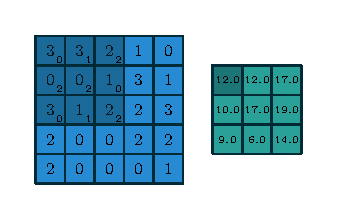
\includegraphics[width=0.7\textwidth]{numerical_no_padding_no_strides_00.pdf}
    \caption[A convolutional operation] {An example of a convolutional
    operation. The image has 5 pixels length and width. The convolutional
    filter has size 3$\times$3. The elements are multiplied together and
    summed to the amount in the top left cell in green. The next step would
    shift the convolutional layer one pixel to the left.  Image source:
    ~\cite{dumoulin2016guide}\label{fig:convolution}}
\end{figure}

To stack layers together for deeper models, there are three  additional core
components. First, to allow the model to find non linear relationships, models
will often include a non linear \textit{activation} function after the dot
product and before the next step. Common activation functions include the
\texttt{sigmoid, tanh and ReLU} functions. The \texttt{ReLU} is popular
because it is fast and effective. For an output $x$, the
\texttt{ReLU} is $\max\{0, x\}$.

Second, to reduce the spatial size of the output, a \textit{pooling} reduces a
$\ell\times\ell$ patch of the output to a single number, using the $\max$
operator (See Figure~\ref{fig:maxpooling}). Pooling layers act to extract
what, at the expense of local details.  Pooling reduces the amount of
parameters in the model and helps against overfitting the data.

\begin{figure}
	\centering
    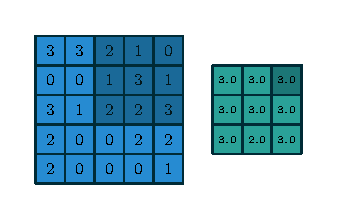
\includegraphics[width=0.7\textwidth]{numerical_max_pooling_02.pdf}
    \caption[A max pooling operation] {An example of a max pooling operation.
    The image has 5 pixels length and width. The pooling filter has size
    3$\times$3. The maximum value of the image within the window is passed to
    the output cell in green. The next step would shift the convolutional
    layer one pixel to the left. Image source: ~\cite{dumoulin2016guide}
    \label{fig:maxpooling}}
\end{figure}

The bulk of a convolutional neural network is stacking these layers on top of
each other. After stacking these layers on top of each other, we flatten the
output to a one dimensional layer. Dense layers are added on top. Once we
understand these building blocks, coding them is straight forward (see
Figure~\ref{alg:simple_convnet}).

\begin{figure}
\begin{minted}[
frame=lines,
linenos
]{python}
    # load libraries
from keras.models import Model, Sequential
from keras.layers import Conv2D, MaxPooling2D
from keras.layers import Flatten, Input
from keras.layers import LSTM, Embedding, Dense

model = Sequential()
    # add first convolutional layer with 
    # 64 filters of size 3 x 3
    # and padding to retain image size
    # and ReLU activation function
model.add(Conv2D(64, (3, 3), 
          activation='relu', 
          padding='same', 
          input_shape=(224, 224, 3)))
    # add second convolutional layer with 
    # 64 filters of size 3 x 3
    # and ReLU activation function
    # no padding
model.add(Conv2D(64, (3, 3), 
          activation='relu'))
    # add pooling
model.add(MaxPooling2D((2, 2))
model.add(Flatten())
model.add(Dense(4096, activation='sigmoid')(inputs)
model.add(Dense(10, activation='sigmoid')(inputs)

\end{minted}
    \caption[A simple convnet in\texttt{Keras}]{A simple convnet in\texttt{Keras}. This model
    has two convolutional layers with ReLU activation functions, a max
    poolution layer and a dense layer to predict 10
    classes.\label{alg:simple_convnet}}
\end{figure}
\subsection{Training models}

The question is then: how to train these (hundreds of) millions of parameters?
The high level answer has two steps. First, observe the \textit{error}
between predictions and actual labels. The \textit{loss} is a function of the
error. For instance, one loss is the error squared. The second step is to pass
this loss through the model, updating parameters that cause the most loss.

This second step is known as \texttt{gradient descent}. Gradient descent is a
way of finding the minimum of a function, in our case, the loss function. We
take the gradient of the loss function and update the weights by the negative
of the gradient (see Figure~\ref{alg:graddesc}). 

\begin{figure}
\begin{minted}
[
frame=lines,
linenos
]{python}
while True:
  weights_grad = evaluate_gradient(loss_fun, 
                                   data, 
                                   weights)
    # perform parameter update
  weights += - step_size * weights_grad
\end{minted}
    \caption[Pseudo code for basic gradient descent]{Pseudo code for basic
    gradient descent. First, we calculate the gradient of the loss function
    with respect to the model weights. We then use this to modify the model
    weights. Source:~\cite{CS231n}\label{alg:graddesc} }
\end{figure}

Since we often train on many thousands (millions) of images, we cannot compute
this in memory. Insted, a small batch of images is used and the model updated.
This is called \texttt{batch gradient descent}. There is also stochastic
gradient descent for  batches of size one observation. With enough batches,
we obtain good results.

We don't have to hard code the \texttt{evaluate\_gradient} function, we can
rely on libraries to do this for us. We saw this in Figures~\ref{alg:linreg}
and~\ref{alg:linearimage} above. We have the \texttt{sgd}, or stochastic
gradient descent optimiser and the \texttt{rmse} or root mean squared error
loss function. 

% Some evidence that adaptive weight mechanisms perform better on test set and
% worse on training set (https://arxiv.org/abs/1705.08292). I.e. worse
% generalisation.

There many options for both the optimiser and the loss function. The
development of optimisers is an ongoing area of research
(e.g.~\cite{wilson2017marginal}). Despite the choice, default options will be
more than fine for experimentation. Results may vary so it can be worthwhile
testing out different optimisers. Loss functions are selected by the problem
at hand. For regression, root mean squared error loss functions are most
common. For classification, categorical cross entropy is most common. 

\section{Literature}

The above section is a quick introduction to convolutional neural networks. We
go deeper in this section, focusing on key results in image classification,
object detection and segmentation. These problems nest each other: to detect
an object, a machine needs to know what the object is (classification) and
where it is. To segment and image, the machine needs to know where the object
is (detection and classification) and where the boundaries of these objects
are. We begin with a classic of convolutional neural networks, VGG Net.

% Measure evolution --> performance on standard tasks

\subsection{If you understand VGG-net, you're 80 per cent there}

VGG Net~\cite{SimonyanZ14a} came second in LSVRC 2014 (losing to GoogleNet see
below) with a 7.4 error rate on Image Net. Although not the best performing
model, it has a simple architecture and is perfect for beginners. The
architecture is a repeating set of convolutional layers to extract spatial
imformation, activation layers for non linearities and max pooling to reduce
information. There are two versions of VGG net, one with 16 and one with 19
layers. VGG net has around 140 million parameters. Most of these are in the
fully connected layers. 

VGG net is widely used as a \textit{feature extractor}. VGG net can extract
features by taking an arbitrary image and setting the output at the flattening
stage. That is, we remove the fully connected layers (or `top') of the model
and reduce the image to a vector. The vector retains some high dimensional
representation of the image that can be used in a standard classifier, for
example a logistic regression model. The original VGG net weights are used,
and no training is undertaken. This is a common practice and can be used to
train models on very few observations.

\textbf{Recommendation:} \textit{when there are only a few observations that you can
label (for instance, water bodies) at low cost, extract information from
satellite/drone images using VGG net. Run a logistic regression model using
extracted information as inputs and labeled images as outputs.}

In Figure~\ref{alg:vgg} we download the model on line 6. The full code of VGG net
is in the appendix.\footnote{There are only 4096 layers in this version of the
model}. In this block we download the whole model so that we can use the model
to predict what's in the image (TO DO: run an example here). If we want to
extract features, we can change the argument \texttt{include\_top} to be
\texttt{False}. Rather than a list of object class weights, the output of
\texttt{model.predict()} will be a 4096 dimensional vector. We can store these
for use in another model.

\begin{figure}
\begin{minted}[
frame=lines,
linenos
]{python}
from keras.applications.vgg16 import VGG16
from keras.preprocessing import image
from keras.applications.vgg16 import preprocess_input
import numpy as np

model = VGG16(weights='imagenet', include_top=True)

img_path = 'remote_area_example.jpg'
img = image.load_img(img_path, target_size=(224, 224))
x = image.img_to_array(img)
x = np.expand_dims(x, axis=0)
x = preprocess_input(x)

features = model.predict(x)
\end{minted}
    \caption[Using VGG16 in \texttt{Keras}]{Using VGG16 in \texttt{Keras}. On
    line 6 we import the model architecture and model weights.\label{alg:vgg}}
\end{figure}

\subsection{Object detection}

There are many other object classification models, from the groundbreaking
LeNet~\cite{lecun1998gradient} to recent ensemble models. We focus on a three
key papers that provide additional tools have helped to drive progress in
object classification (see Figure~\ref{fig:imagenetoverview}).

\begin{figure}
    \centering
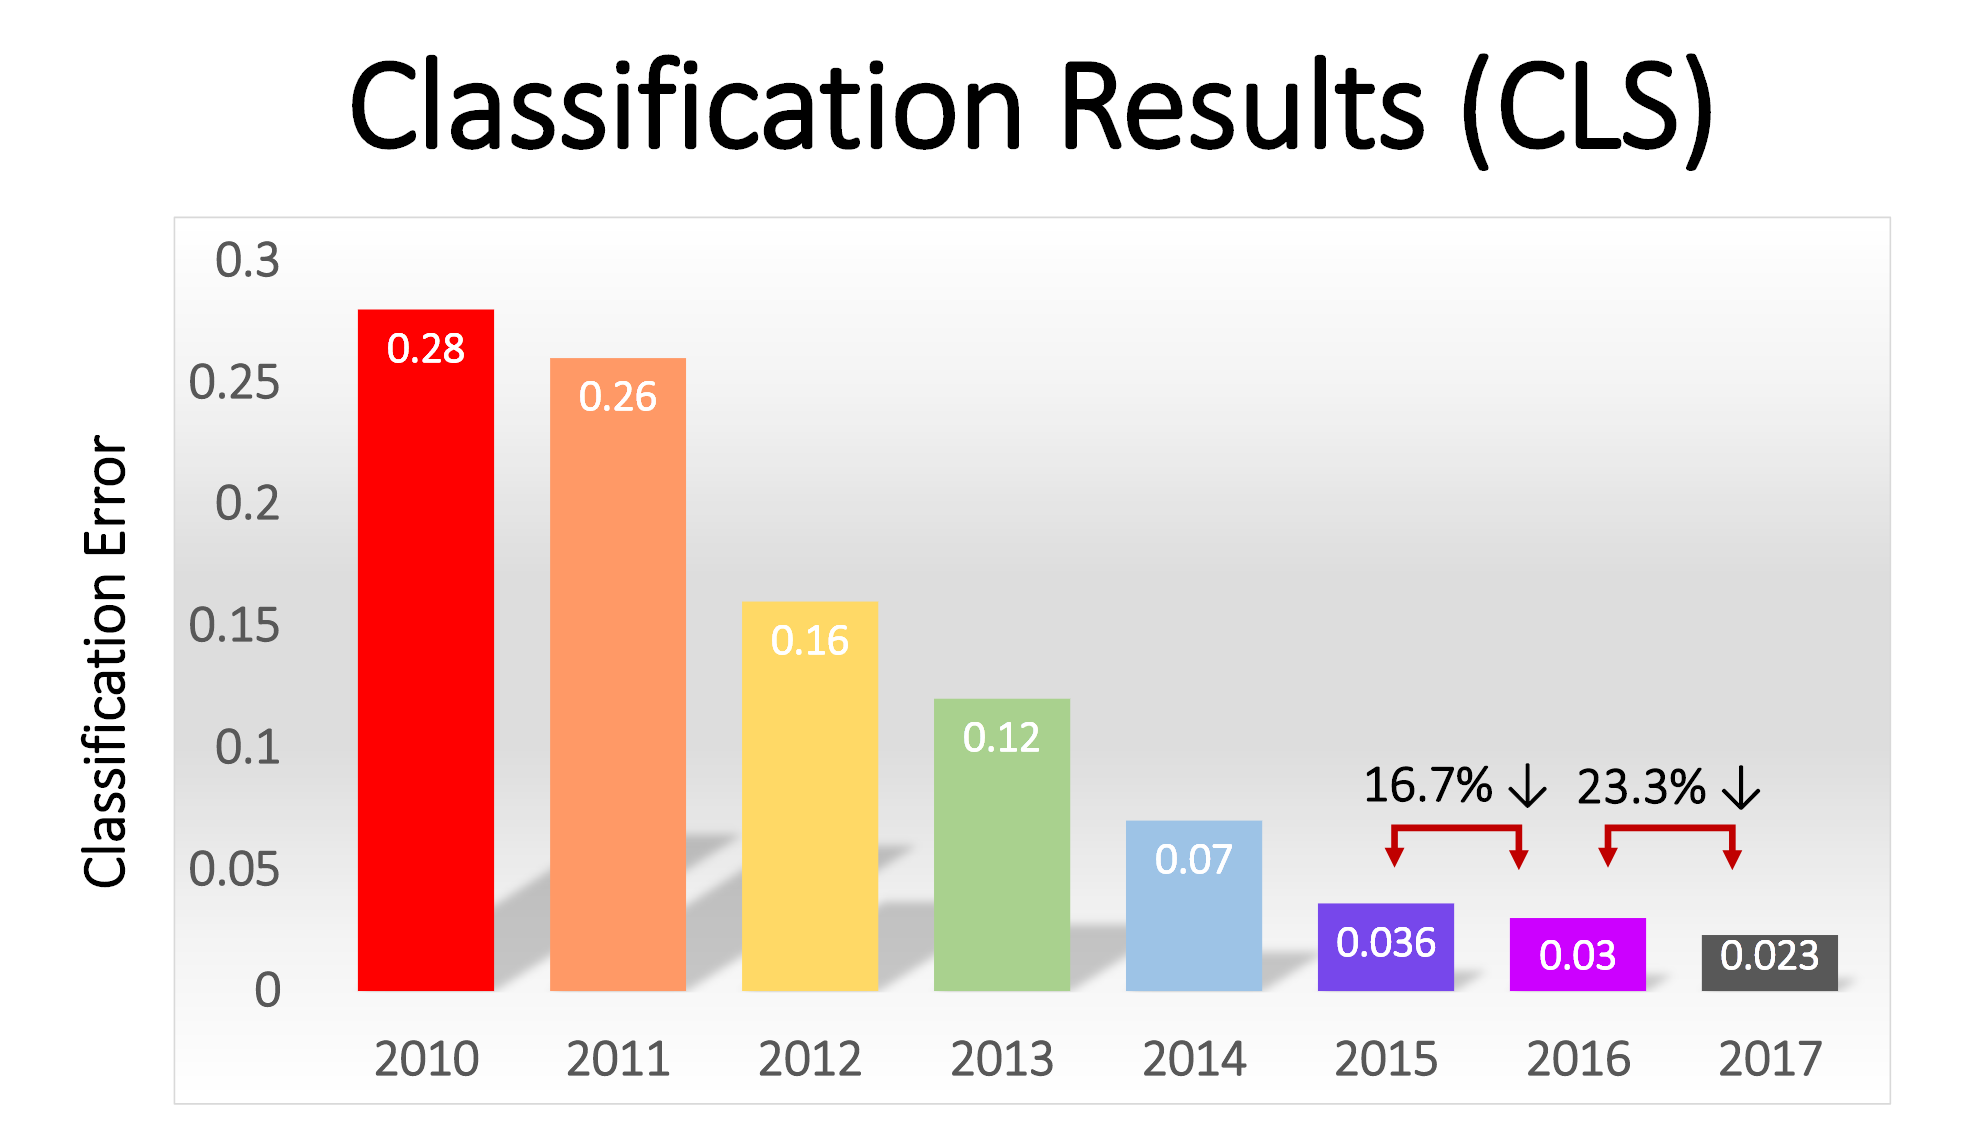
\includegraphics[width=0.7\textwidth]{imagenet_classification_results.png}
    \caption[ImageNet classification results, 2010--2017]{ImageNet
    classification results, 2010--2017. We see that the error rate dropped
    rapidly over 2011--2015. Source: Image Net
    Overivew\footnote{\url{http://image-net.org/challenges/talks_2017/ILSVRC2017_overview.pdf}}\label{fig:imagenetoverview}}
\end{figure}

We begin with AlexNet, which won ImageNet in 2012~\cite{NIPS2012_4824}.
AlexNet features three innovations which are still in use today. To begin,
AlexNet was the first model to `go deep', with five convolutional layers.
Second, the model used the \texttt{ReLU} activation function. Last, to prevent
\textit{overfitting}, or having a model memorise training data and exhibit
poor performance on new data, AlexNet used \textit{dropout}. Dropout worked by
randomly setting the value of some parameters to zero during training. This
way, the model could not rely on specific parameters to predict object
classes. Instead, the model has to `spread' this information across
parameters.

Models went deeper over the next few years, but a puzzle arose: performance
did not rise -- infact sometimes performance dropped -- with additional
layers. This was a puzzle because models could simply pass on the same output
through multiple layers rather than having degraded performance. This insight
resulted in the residual learning framework that passes both the input $x$ and
the output of a layer $f(x)$ to the next layer. With these skip connections
the model can choose to discard elements of the modified layer output if
elements do not help in prediction. An additional innovation is the lack of
fully connected layers at the end of the model. These innovation allowed ResNet
to have 152 layers and have lower model complexity~\cite{he2016deep}. ResNet
won ILSVRC
2015.\footnote{\url{https://towardsdatascience.com/squeeze-and-excitation-networks-9ef5e71eacd7}}

The current state of the art involves creating a model out of an ensemble of
models. The winner of the 2017 ImageNet challenge used ensembles and an
innovation called `Squeeze and excitation'~\cite{wmw}. Squeeze-and-excitation
networks weight the information across image channels. That is, if the red
image channel helps with prediction more (say, for fire trucks), the model
will learn to use channel to make predictions. SENets lowered the ImageNet
classification error rate by almost 25 per cent.  That said, the object
detection problem for image net is 99 per cent solved.  Research is
progressing on more challenging problems. There is still a lot of room to
improve for aerial or satellite imagery. In particular, SENets could exploit
the 5-10 bands of information that comprise satellite images. We discuss this
in section X and now move to detection where an object is.

Evidence that the number of bands does not for building detection~\cite{2017Panchromatic}

The next step after identifying if an object is in an image is pointing out
where the object is. This challenge, to ``detect a \textit{potentially large
number of object instances with varying sizes in the same image} using a
limited amount of computing resources.''~\cite[Their emphasis]{NIPS2013_5207}
is known as object detection. Models that solve this problem will be useful for identifying
where key sites --- like damaged roads --- are.

A brute force, basic model is to slide a classifier across an image. Since
this model will have to run multiple times over a single image the model will
be very slow. 

An early innovation is to treat localisation as a regression
problem~\cite{NIPS2013_5207}. This model uses a small standard convolutional
neural network, but instead of a softmax classifier layer, the model uses a
regression layer to output a binary mask: 1 for inside a bounding box, 0 for
outside. One problem was that most of the image is outside the bounding box,
so a model can learn to only output zeros. The authors increase the weights of
non zero outputs to overcome this problem. Overall, there are five networks:
one for box predictions, four others for where the {top, bottom, left, right}
of the box. As with many of the models to come, the model is `pre-trained' on
a classification task. 

The next innovtion came with regions with CNN features
(RCNN)~\cite{Girshick2014, Girshick2015}. RCNN improved on mAP (mean Average
Precision) by more than 30\%. They get mAP of 53.3\%. Their idea is to extract
some two thousand bounding boxes in a preprocessing step, run a classifier
through these boxes and combine them at the end. They also use supervised pre
training on a large dataset using the VGG net architecture. RCNN is multi
stage, expensive and slow. 

Additional innovations increased the speed of this model.
Fast-RCNN~\cite{Gershick2015} shares features across object proposals rather
than recalculating features for each proposal. The model also features a multi
task loss function for classification and a four dimensional regression for
the bounding box. Faster RCNN~\cite{Ren2017} overcomes the bottleneck of
region proposals with a `Regional Proposal Network' (RPN). The RPN takes
\textit{anchors}, or fixed points in the image, and first classifies whether
there is any object there.  Second, the anchor bounding box is adjusted for a
better fit. FasterRCNN is trainable end to end. So at the end you get a set of
overlapping proposals. If we have two overlapping images, discard one with
lower classification
score.\footnote{https://towardsdatascience.com/squeeze-and-excitation-networks-9ef5e71eacd7}

% \url{https://tryolabs.com/blog/2018/01/18/faster-r-cnn-down-the-rabbit-hole-of-modern-object-detection/}
% Predicing (xmin, xmax, ymin, ymax) is hard. For instance, how to enforce
% xmin < xmax
% Useful overview:
% \url{https://blog.athelas.com/a-brief-history-of-cnns-in-image-segmentation-from-r-cnn-to-mask-r-cnn-34ea83205de4}

% \textbf{Mask RCNN}~\cite{he2017}

% We can do segmentation as well! Have a third branch that allows segmentation. 

% But there is a slight misalignment between bounding boxes and pixels because
% of pixel integers. The original image is say 200 $\times$ 200 and the feature map is
% say 30 * 30. So to select the top 15*15 corner we need 15 * 30 / 200 $\approx$
% 2.25 pixels. RoIPool uses 2$\times$2. RoIAlign (this paper's innovation) uses
% bilinear interpolation to get an idea of what the 2.25th pixel is.


% \textbf{R-FCN}~\cite{NIPS2016_6465}

% The above apply a costly per region subnetwork hundreds of times :(

% \textit{Translation invariance} - the object can be anywhere in an image for
% correct classification

% \textit{Translation variance} - if we move the object, the bounding box should
% change. 

% Use an RPN for proposals.

Although these innovations increased the speed, detection was still slow. The
You Only Look Once (YOLO) series of models model~\cite{redmon2016yolo} traded
off accuracy for speed.\footnote{For a video showing the speed at which YOLO
can work, see \url{http://www.youtube.com/watch?v=NM6lrxy0bxs}} YOLO divides
an image into a grid. For each grid cell, there are a number of bounding
boxes. The output of the model is 5 elements: four spatial components that
modify the shape of a candidate bounding box and a measure of confidence.  The
model then applies a classifier. The model uses Google's LeNet as a base model
and shows good performance in new domains. YOLO version 2 improved performance
through pretraining the model on the ImageNet classification task.

Because of this and the model's spend, YOLO might be useful for a first pass
over large areas of satellite images. The limitations of YOLO is that it is
not the best for identifying many tightly connected objects (this is because
of the hard coded grid size and number of bounding boxes per gridcell).
Generalisation doesn't work well with different aspect ratios. 

A recent extension modifies YOLO for satellite images~\cite{YOLT}. In addition
to image augmentation, the authors have two innovations that help identify
images in satellite images. First, they use upsampling and ensemble models
at different scales to capture small images. For instance, one classifier for
airports and another for aeroplanes. Second, they define a new network
architecture with a denser final output for smaller bounding boxes.


An alternative to YOLO is Single Shot Detection (SSD) ~\cite{liu2016ssd}. SSD
is similar to YOLO but uses multiple grid sizes. SSD was faster and stronger
thand YOLO v1. The author has used this for building detection using satellite
images (under review).

\subsection{Image segmentation}

The final task we investigate is image segmentation. The challenge here is to
outline the boundary of the object (see Figure X). In one sense this is a
simple extension of classification: but one prediction per pixel rather than
one prediction per picture. Segmentation would be useful in tracing out road
paths and distinguishing regions with damaged properties versus non damaged. 

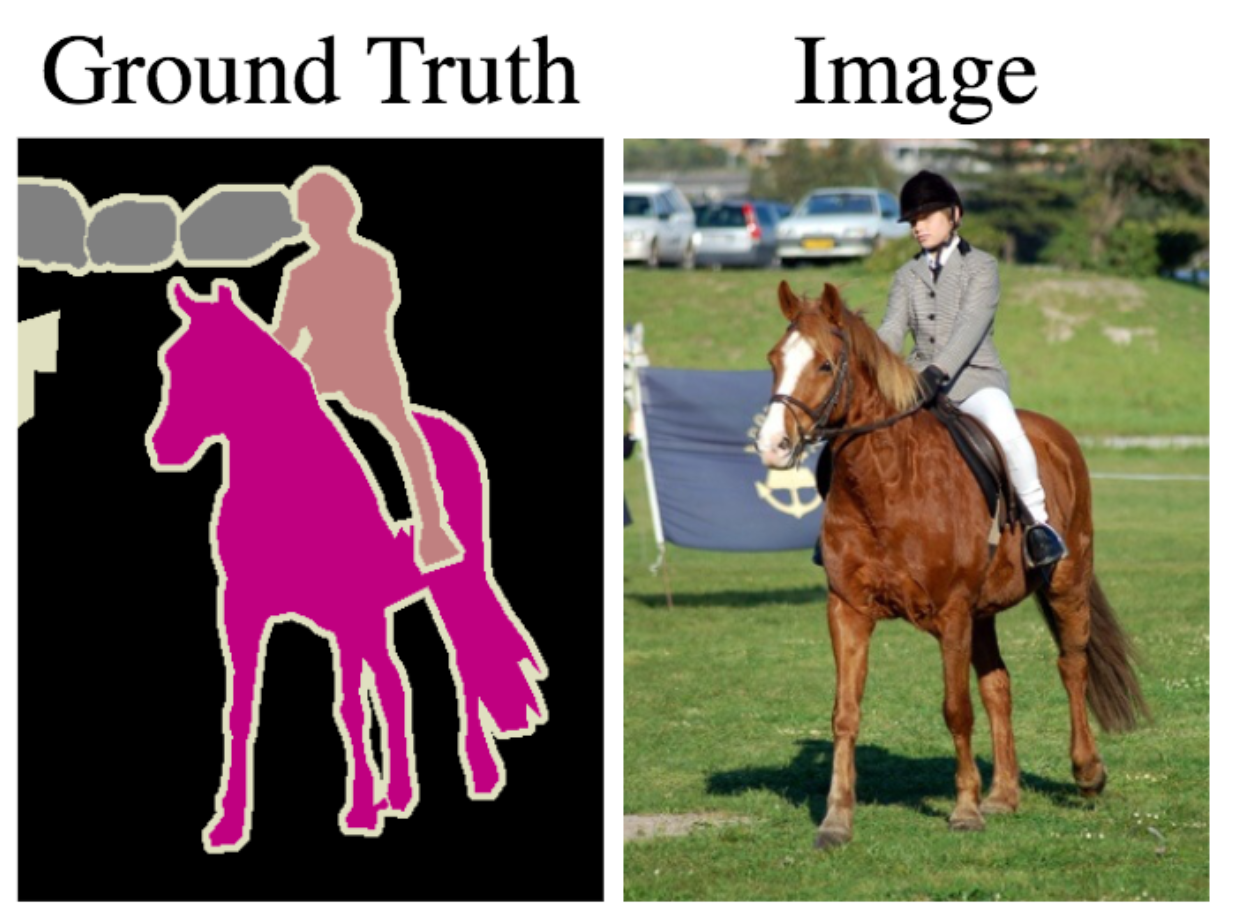
\includegraphics[width=0.5\textwidth]{Figures/segmentation-example.png}

A common metric in segmentation problems is the mean intersection of
prediction and ground truth over their union. When the prediction is perfect,
then the intersection equals the union and the metric is 1. When no predicted
pixel overlaps with the ground truth, the metric is 0. Calculating this
measure for each image then averaging is preferred to averaging over the test
set~\cite{csurka2013good}.

% In fact, early models ran a class model over each pixel~\cite{NIPS2015_5852}. 
With segmenation, there is a tension between `semantics and location.'
\textit{Semantics} is the question of what, \textit{location} asks where.
Local information helps answer the former and global information helps answer
the latter. This need for two types of information gave rise to complicated
models prior to the era of fully end to end differentiable models. This
tension also explains the innovations beyond basic CNNs used for
classification.

\cite{long2015fully} developed the first end to end trained CNN for
segmentation.\footnote{BTW, very good write up on
convnets.~\cite{long2015fully}} \cite{long2015fully}'s insight was to think of
a fully connected layer as a 1 x 1 convolutional layer that covers the whole
image. Using a standard convnet (e.g. VGG net) did not work well as by the
time you've gotten to predicting a pixel, you've lost a lot of the information
on the surrounding pixels. The authors get around this by bringing
intermediate layers back into the prediction. A skip architecture brings
intermediate layers back into prediction, allowing the model to combine
coarser semantic information and finer appearance information. 

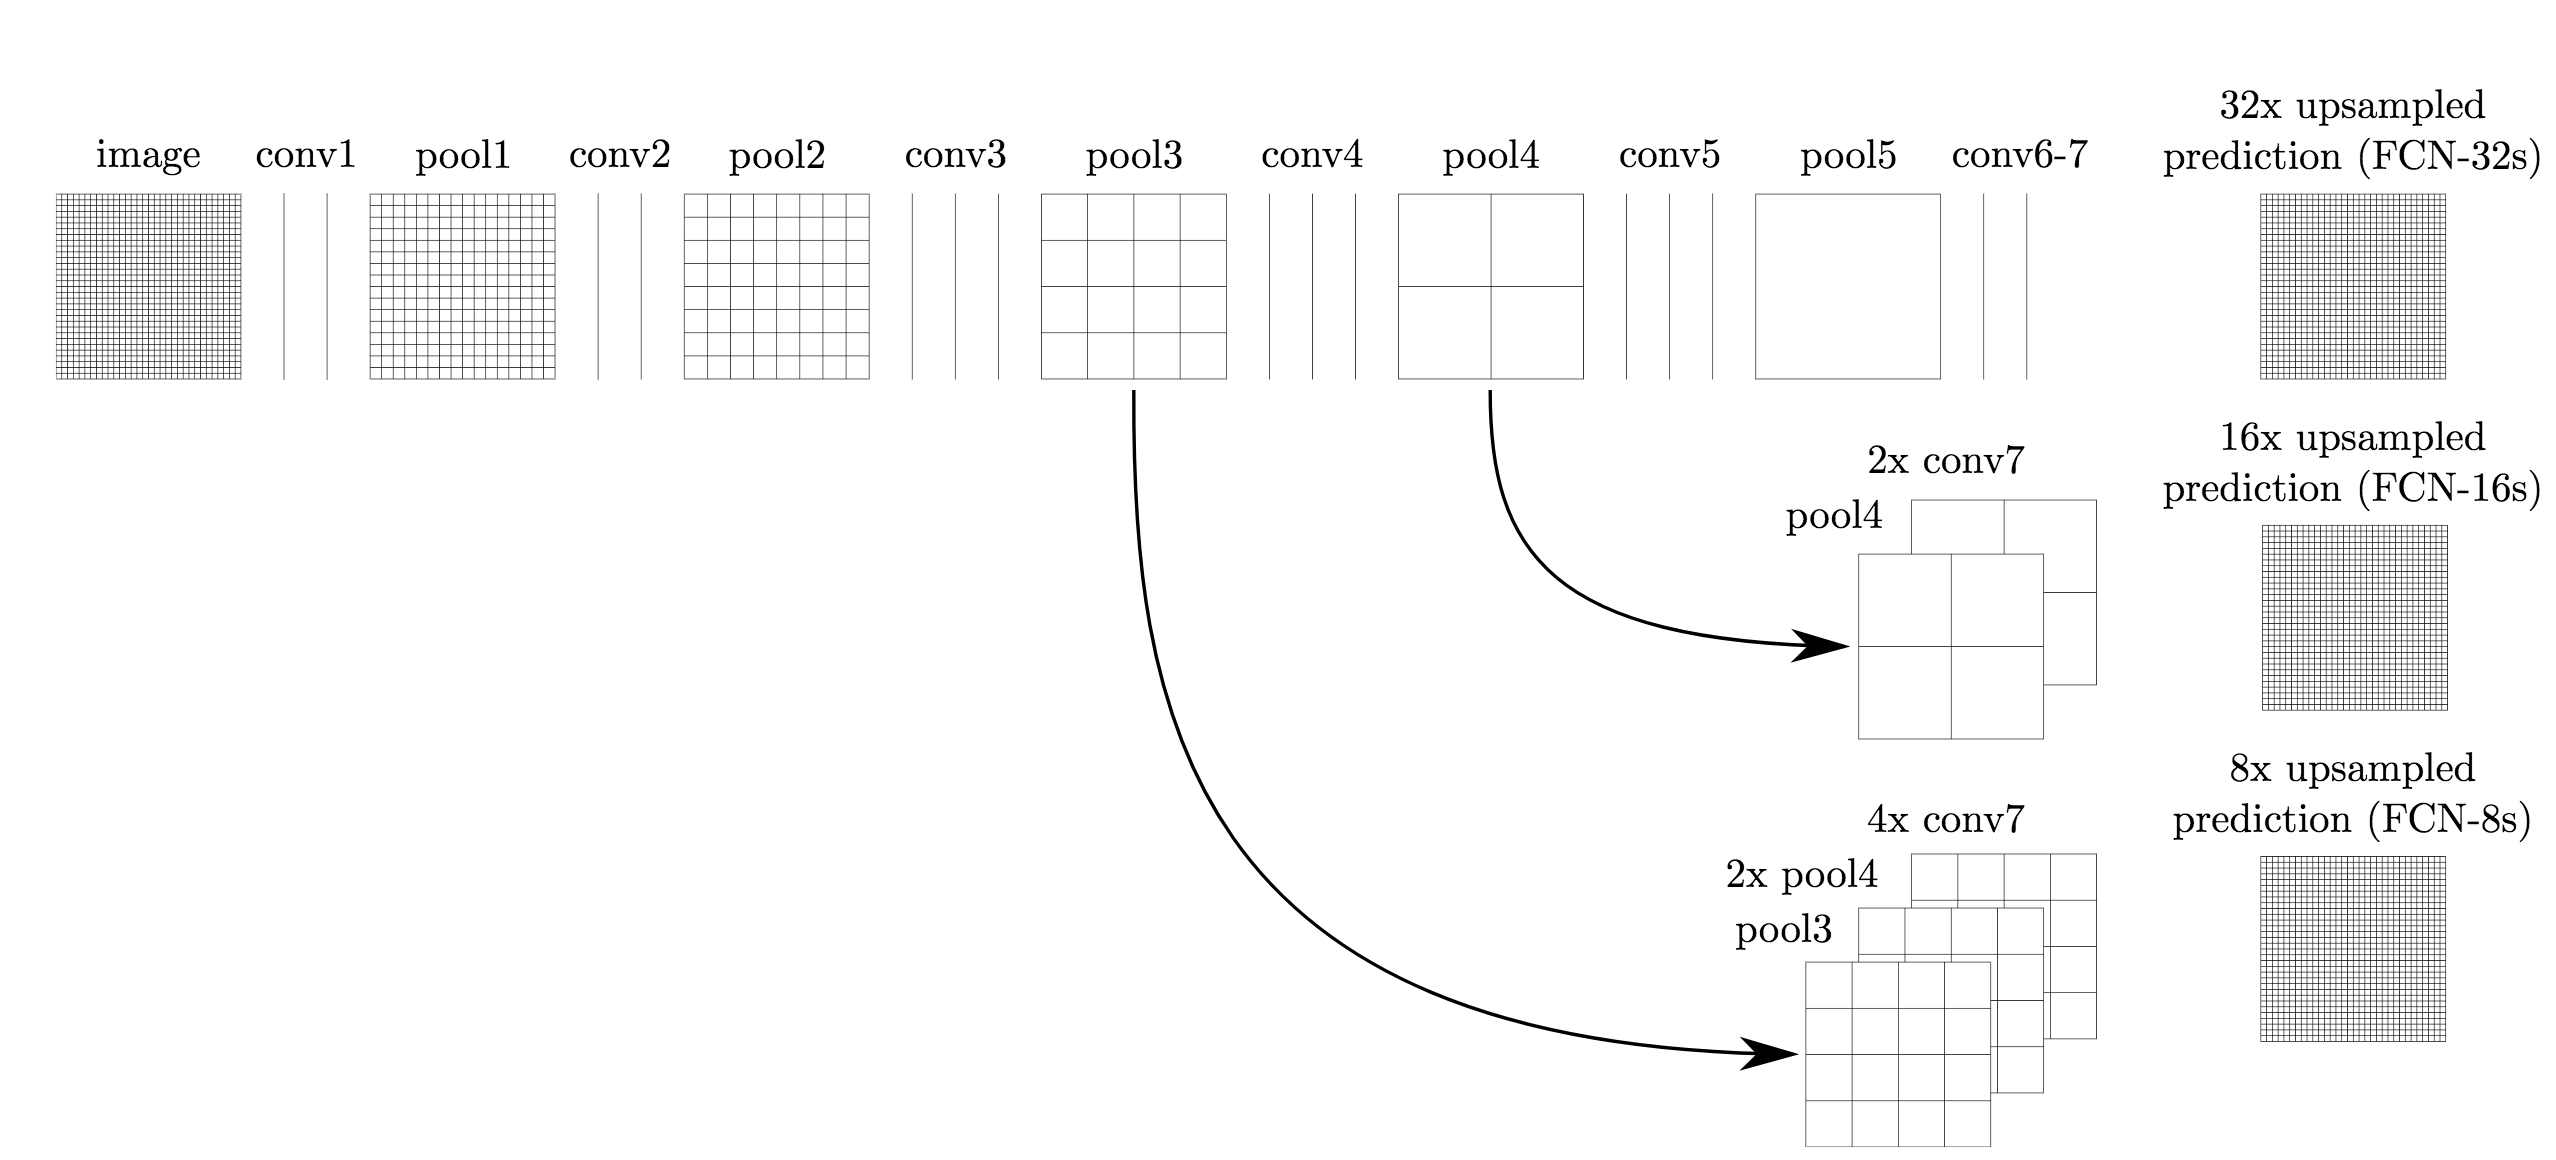
\includegraphics[width=0.75\textwidth]{Figures/skip-segmentation.png}

The output of FCN was still too coarse. The solution was to bring in more
skips. Many models do this~\cite{segnet, unet}.\footnote{If you like, you can
always combine the two~\url{https://github.com/ykamikawa/Seg-UNet}}
U-Net~\cite{unet} uses a convnet to \textit{encode}, or extract features. A
\textit{decoder} network then converts these features into a per pixel
classification. Because the feature is a small dense representation, the
decoder network must \textit{upsample} -- or `blow up' -- the image from the
dense representation.  Because upsampling is sparse, the output from the
corresponding encoding stage is concatenated to the dense representation. A
benefit of UNets is that we can use any pretrained network to encode the data.
Unets are commonly used in the data science community. Segnet uses a similar
architecture, but rather than the memory intensive step of transfering
features, the model transfers indices from the maxpool steps.

An alternative attack on max pooling is to discard them and use components
that compress class information while retaining
location~\cite{chen2018,dilated2017}.  These components, called
\textit{atrous} convolutions, generate low to mid resolution outputs. These
models require an additional step to refine the segmentation. Conditional
Random Fields (CRF) are used most often.  CRFs take the output of convent and
image and tries to map the convnet output to the rgb together. (e.g. looking
for edges).

(Dilation figure here).

\begin{minted}{python}
model.add(Conv2D(..., dilation_rate=2)) 
\end{minted}

A further alternative uses interpolation. Mask RCNN~\cite{he2017} extends
faster RCNN by adding a branch to the model for pixel level classification.
Since the output of the CNN is smaller than the ground truth image, some form
of \textit{upsampling} or increasing the size of output images is required.
Mask RCNN achieves this by using interpolation. Say our image size is 512 x
512, we are proposing a region in the top left 25 x 25 pixel corner, and
feature map is size 30 x 30. Then our region of interest is 25 $\times$ 30 /
512 $\approx$ 1.46 pixels of the feature map. A naive implementation would use
integer division for a region proposal of 1 pixel. Mask RCNN uses bilinear
interpolation to estimate what the 1.46th pixel would look like.


% outputs. A

% Repeated pooling shrinks output size. Long range skip connections. Use
% \textit{chained residual pooling} which  is  able  to  capture
% background context from a large image region. It does so  by  efficiently
% pooling  features  with  multiple  window sizes and fusing them together with
% residual connections and learnable weights

% \paragraph{Learning to segment object candidates}~\cite{NIPS2015_5852} 

\section{Analysis with satellite images}

We now look at what has been done with satellite images. There are three
branches of knowledge we can look at. First, there is the academic literature.
Second, data science competitions. Last, we have industry. In this last branch
we can only make educated guesses at how.

Much of the academic literature takes a pre-trained convnet or common
architecture and trains the model on the task at hand. Two papers have focused
on mapping poverty~\cite{babenko2017poverty,Jean79}. \cite{babenko2017poverty}
use satellite images, land use maps and household survey data to map
poverty in Mexico.\footnote{There are two authors working for the World Bank.}
The authors use GoogLeNet and VGG net, but find had best out of sample
performance. They also trained a model using RGB bands and near infrared band.
Because ImageNet models use the three RGB bands, the model had to be retrained
from scratch.  Around fifty per cent of variation in local poverty can be
predicted through satellite images and a convnet alone. This increases to
around sixty per cent when they include land use cover as a feature. It
is not clear from the paper how they include land use cover information
maps. It does not seem to be a feature layer, perhaps it was used as a
regression input with the convnet output.

\begin{equation}
\textup{composite prediction} = \alpha + \beta\textup{convnet output} + \phi\textup{land use}
\end{equation}

\cite{Jean79} estimate poverty across Sub Saharan Africa. Since ground truth
values are difficult to come by, they use night lights as a proxy. They fine
tune a pretrained convnet (VGG 8 layer) to predict night lights. These
features are fed into a ridge regression model (LASSO) to estimate poverty
taken from household surveys. The satellite data is taken from the Google
Static Maps API. Pixels are approximately 1km square. The model's transfer
learning is promising. Figure X shows the average $r^2$ for models trained on
one country and evaluated each country.

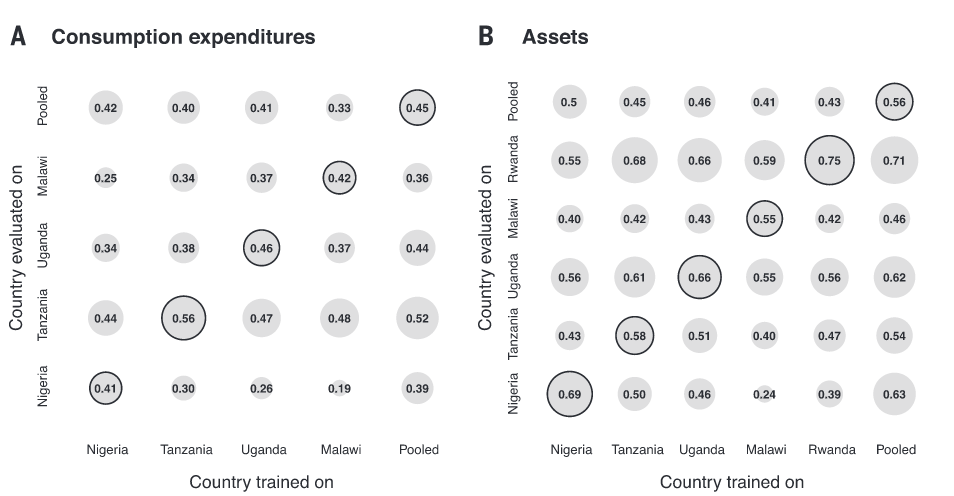
\includegraphics[width=0.7\textwidth]{transfer-learning-poverty.png}

A similar strand of research maps population~\cite{doupe2016, robinson2017}.
\cite{doupe2016} map population in Kenya and Tanzania using a VGG-net style
architecture. The authors exploit all eight landsat bands by retraining a
model from scratch. Because population across satellite images follows a power
law, the log of popualtion is estimated.~\cite{robinson2017} also train their
own model. They use a two step procedure to obtain raw estimates for
population. The first gets coarse values at the pixel level. These are
combined at the county level. The results are directly interpretable as
population estimates. Facebook~\cite{facebook} are also estimating
population. This seems to be a building segmentation map and populations are
distributed throughout the area inferred by the segmentation map. In addition,
they use segmenting tools to identify roads~\cite{demir2018}.

A problem with satellite images is that they are either free and low
resolution or expensive an low resolution. In the past few years, data science
competitions have been organised around small, high resolution datasets. The
two SpaceNet challenges asked participants to segment roads, buildings and
water bodies, amongst others.\url{https://github.com/SpaceNetChallenge}

In the first edition, the test challenge was to predict buildings in Rio de
Janiero, Brazil. This is particularly challenging because buildings in Rio are
small and densely built. Four of the top five entries used convnets. Second
place used SSD, third MNC whereas forth and fifth trained their own model.
Fifth place in particular placed a large emphasis on image augmentation. The
winner used a sequence of well trained random forest models.

In the second edition, additional cities were added. These cities (Las Vegas,
Paris, Shanghai and Khartoum) all have a different built infrastructure. The
winner used U-Net. To use all the spectral bands, the model had to be trained
from scratch. This model did struggle with small and L shaped buildings. The
second and third places used models based on the chained random forests models
that won the first edition. There is a new
competition\url{http://deepglobe.org/challenge.html}.


\subsection{Applications in industry}

Many industries use satellite data to generate information. Unfortunately, we
do not have access to proprietry methods; however, understanding applications
may assist in generating ideas. Common applications include crop monitoring
and forecasting,\footnote{\url{https://telluslabs.com/}} water cover and
use,\footnote{\url{https://www.vandersat.com/}} 
car park occupancy rates (consumer demand) and oil
reserves\footnote{\url{http://www.orbitalinsight.com/}}. Of note is the
insurance industry, who use satellite images for predicting claims amounts,
and identifying damaged or unaffected assets. As one would expect, the
intelligence community and associated research groups are doing work
too.\footnote{For instance, CosmiQ
(\url{http://www.cosmiqworks.org/space-30/}) have developed a time series
model to map infrastructure after a hurricane~\cite{cosmiq} and a tool to
create your own time series from satellite
imagery~\url{https://github.com/CosmiQ/CometTS}}

Consulting companies~\cite{CosmiQ,Satellite}
https://www.spaceknow.com/satellite-ai/

\subsection{NGO applications}

\cite{2016Burma}: HRW used before and after photos to identify burned buildings in
Rohingya villages throughout Burma. Uncertain how they did this.

\cite{2015Nigeria}: Amnesty International used satellite images to identify
buildings and villages attacked by Boko Haram in Nigeria.
Before and after "change detection"
False color image analysis to track distruction. Also used this for 2011 Oil Spill
in Niger~\cite{Koettl2011}j
Identify mass graves in Afghanistan~\cite{2013AAAS}. Locations known prior to
analysis.
For more applications, see~\cite{2014Human}.

For more use on using satellite analysis:
~\cite{Satellite,Making,2018High-Resolution}

\section{Satellite data}

There are many sources of satellite imagery.\footnote{The following URLs
provide a good list as of July 2018:
\url{https://gisgeography.com/free-satellite-imagery-data-list/}
\url{https://docs.google.com/spreadsheets/d/1oFY_TX5QRFyAAu-nxeClnOFB1epSlSDWEHoMalvv0Qs}}
Satellite imagery is expensive, but free or limited options are available. FOr
isntance, both LANDSAT and the Copernicus mission images are free of charge and
available through the USGS Earth
Explorer\footnote{\url{https://earthexplorer.usgs.gov/}} and the Scientific
Data Hub\footnote{\url{https://scihub.copernicus.eu/dhus/}} or the
Google Earth Engine.\footnote{\url{https://earthengine.google.com/}} LANDSAT
has the benefit of a forty year history of images, although at 30m (15m
panchromatic) the resolution is course. The Copernicus Programme's Sentinel
satellites have a resolution of 10m. At these resolutions, individual
buildings will be difficult to isolate.

We know that image resolution matters~\cite{2017The}. It's difficult with the
naked eye to locate a 10 square meter building with 10 square meter pixels.
For the most part, higher resolution imagery typically costs money. For
humanitarian and research purposes, small datasets can be provided. For
instance, Planet and Satellogic have researcher and humanitarian
access~\cite{Planet,Satellogic}. I would not be surprised if other providers
matched this offer. In addition, Google maps and Bing Maps have APIs that
allows users do download a limited amount of  undated high resolution images.
The images have a watermark which can easily be cropped out.
Table~\ref{tab:meinetabelle} presents an overview of high resolution image
providers.

\begin{table}[htb]
\caption{A list of satellite imagery providers}
\begin{tabular}{lcr}
Provider & Free & Description \\
\hline
    Planet & Limited & 3--5m imagery anywhere in the world \\
    Satellogic & Limited & 30 bands, 30m resolution \\
    UrtheCast & N & 0.75m resolution, video available \\    
    Digital Globe & N & Global coverage, 30 cm resolution \\ 
    Bing & Y & High resolution, undated \\
    Google & Y & High resolution, undated \\
\end{tabular} 
\label{tab:meinetabelle}
\end{table}

\subsection{Labelled data}

Training models requires labelled data. One option is to do this by hand or
outsource to services like Mechanical
Turk.\footnote{\url{https://www.mturk.com/}} For drone data or specific
objects to detect, this is a good option. For buildings, roads or waterways,
there are a few datasets of use. Some of these are down, but may still be
available through other researchers, or asking the organisers.

First, there is the Spacenet challenge
data.\footnote{\url{https://spacenetchallenge.github.io/datasets/datasetHomePage.html}}
This data appears to be down at present. The data consists of very high
resolution (30--50cm) images of five cities. The data contains labels of
buildings, trees, cards, roads and waterways. More labelled urban environments
can be found in Urban Environment
dataset.\footnote{\url{https://github.com/adrianalbert/urban-environments/tree/master/dataset-collection}}
For labels, there are two good sources. First, the Urban Atlas
project.\footnote{\url{https://www.eea.europa.eu/data-and-maps/data/copernicus-land-monitoring-service-urban-atlas}}
This project is used in the Urban Environment dataset. A second option is
OpenStreetMap.\footnote{\url{https://www.openstreetmap.org}} These maps are
created by volunteers, much like wikipedia. Your mileage may vary with
building accuracy. 

\section{Recommendations}

\appendix

\section{VGG net}
https://gist.github.com/baraldilorenzo/07d7802847aaad0a35d3

\begin{minted}{python}
from keras.models import Sequential
from keras.layers.core import Flatten, Dense, Dropout
from keras.layers.convolutional import Convolution2D, MaxPooling2D, ZeroPadding2D
from keras.optimizers import SGD
import cv2, numpy as np

def VGG_16(weights_path=None):
    model = Sequential()
    model.add(ZeroPadding2D((1,1),input_shape=(3,224,224)))
    model.add(Convolution2D(64, 3, 3, activation='relu'))
    model.add(ZeroPadding2D((1,1)))
    model.add(Convolution2D(64, 3, 3, activation='relu'))
    model.add(MaxPooling2D((2,2), strides=(2,2)))

    model.add(ZeroPadding2D((1,1)))
    model.add(Convolution2D(128, 3, 3, activation='relu'))
    model.add(ZeroPadding2D((1,1)))
    model.add(Convolution2D(128, 3, 3, activation='relu'))
    model.add(MaxPooling2D((2,2), strides=(2,2)))

    model.add(ZeroPadding2D((1,1)))
    model.add(Convolution2D(256, 3, 3, activation='relu'))
    model.add(ZeroPadding2D((1,1)))
    model.add(Convolution2D(256, 3, 3, activation='relu'))
    model.add(ZeroPadding2D((1,1)))
    model.add(Convolution2D(256, 3, 3, activation='relu'))
    model.add(MaxPooling2D((2,2), strides=(2,2)))

    model.add(ZeroPadding2D((1,1)))
    model.add(Convolution2D(512, 3, 3, activation='relu'))
    model.add(ZeroPadding2D((1,1)))
    model.add(Convolution2D(512, 3, 3, activation='relu'))
    model.add(ZeroPadding2D((1,1)))
    model.add(Convolution2D(512, 3, 3, activation='relu'))
    model.add(MaxPooling2D((2,2), strides=(2,2)))

    model.add(ZeroPadding2D((1,1)))
    model.add(Convolution2D(512, 3, 3, activation='relu'))
    model.add(ZeroPadding2D((1,1)))
    model.add(Convolution2D(512, 3, 3, activation='relu'))
    model.add(ZeroPadding2D((1,1)))
    model.add(Convolution2D(512, 3, 3, activation='relu'))
    model.add(MaxPooling2D((2,2), strides=(2,2)))

    model.add(Flatten())
    model.add(Dense(4096, activation='relu'))
    model.add(Dropout(0.5))
    model.add(Dense(4096, activation='relu'))
    model.add(Dropout(0.5))
    model.add(Dense(1000, activation='softmax'))

    if weights_path:
        model.load_weights(weights_path)

    return model

if __name__ == "__main__":
    im = cv2.resize(cv2.imread('cat.jpg'), (224, 224)).astype(np.float32)
    im[:,:,0] -= 103.939
    im[:,:,1] -= 116.779
    im[:,:,2] -= 123.68
    im = im.transpose((2,0,1))
    im = np.expand_dims(im, axis=0)

    # Test pretrained model
    model = VGG_16('vgg16_weights.h5')
    sgd = SGD(lr=0.1, decay=1e-6, momentum=0.9, nesterov=True)
    model.compile(optimizer=sgd, loss='categorical_crossentropy')
    out = model.predict(im)
    print np.argmax(out)
\end{minted}
%----------------------------------------------------------------------------------------
%	BIBLIOGRAPHY
%----------------------------------------------------------------------------------------

\renewcommand{\refname}{\spacedlowsmallcaps{References}} 

\bibliographystyle{unsrt}

\bibliography{review.bib}

%----------------------------------------------------------------------------------------

\end{document}
